% Architecture diagram (vector). Build: latexmk -pdf architecture.tex
\documentclass[tikz,border=2pt]{standalone}
\usepackage[T1]{fontenc}
\usepackage{helvet}
\renewcommand{\familydefault}{\sfdefault}
\usetikzlibrary{positioning,fit,arrows.meta,calc,backgrounds}

\definecolor{awsB}{HTML}{C76A00}\definecolor{awsF}{HTML}{FFF6EA}
\definecolor{gcpB}{HTML}{1A5FC8}\definecolor{gcpF}{HTML}{EEF4FE}
\definecolor{stoF}{HTML}{E9F6EC}\definecolor{stoB}{HTML}{2E7D32}
\definecolor{cmpF}{HTML}{F3EEFB}\definecolor{cmpB}{HTML}{6A4BA8}
\definecolor{extF}{HTML}{F2F2F2}\definecolor{extB}{HTML}{555555}
\definecolor{flow}{HTML}{C62828}\definecolor{rep}{HTML}{00796B}

\tikzset{
  font=\scriptsize,
  box/.style={draw=#1, rounded corners=2pt, align=center, inner sep=2.5pt, line width=0.5pt},
  ctl/.style={box=black!60, fill=white, minimum height=1.0cm},
  sto/.style={box=stoB, fill=stoF, minimum height=0.95cm},
  cmp/.style={box=cmpB, fill=cmpF, minimum height=1.0cm},
  ext/.style={box=extB, fill=extF, minimum height=0.9cm},
  arr/.style={-{Stealth[length=4pt]}, line width=0.6pt},
  biarr/.style={{Stealth[length=4pt]}-{Stealth[length=4pt]}, line width=0.6pt},
  stepn/.style={circle, fill=flow, text=white, inner sep=0.7pt, font=\tiny\bfseries},
  lbl/.style={font=\tiny, align=center, inner sep=1pt},
}

\begin{document}
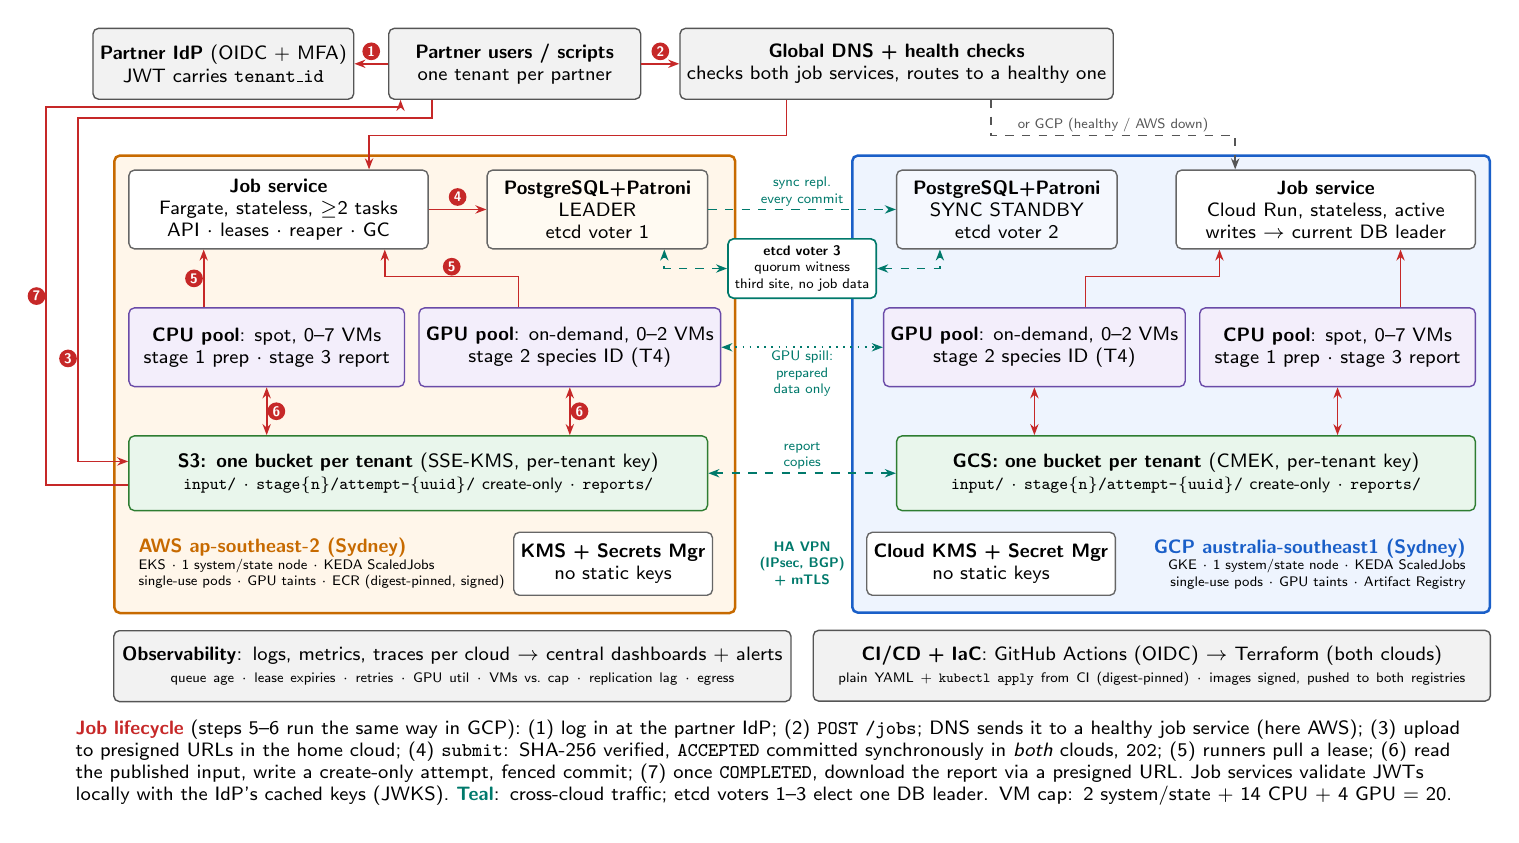
\begin{tikzpicture}

% ================= top row: external services
\node[ext, minimum width=2.8cm] (idp) at (1.45,9.55)
  {\textbf{Partner IdP} (OIDC + MFA)\\JWT carries \texttt{tenant\_id}};
\node[ext, minimum width=3.2cm] (users) at (5.15,9.55)
  {\textbf{Partner users / scripts}\\one tenant per partner};
\node[ext, minimum width=4.4cm] (dns) at (10.0,9.55)
  {\textbf{Global DNS + health checks}\\checks both job services, routes to a healthy one};

% ================= AWS (left)
\node[ctl, minimum width=3.8cm] (jobA) at (2.15,7.7)
  {\textbf{Job service}\\Fargate, stateless, $\geq$2 tasks\\API $\cdot$ leases $\cdot$ reaper $\cdot$ GC};
\node[ctl, minimum width=2.8cm, fill=awsF!60] (dbA) at (6.2,7.7)
  {\textbf{PostgreSQL+Patroni}\\LEADER\\etcd voter 1};
\node[cmp, minimum width=3.5cm] (cpuA) at (2.0,5.95)
  {\textbf{CPU pool}: spot, 0--7 VMs\\stage 1 prep $\cdot$ stage 3 report};
\node[cmp, minimum width=3.5cm] (gpuA) at (5.85,5.95)
  {\textbf{GPU pool}: on-demand, 0--2 VMs\\stage 2 species ID (T4)};
\node[sto, minimum width=7.35cm, text width=7.15cm] (s3) at (3.925,4.35)
  {\textbf{S3: one bucket per tenant} (SSE-KMS, per-tenant key)\\
   {\fontsize{6}{7}\selectfont\texttt{input/} $\cdot$ \texttt{stage\{n\}/attempt-\{uuid\}/} create-only $\cdot$ \texttt{reports/}}};
\node[anchor=west, align=left, font=\tiny] (noteA) at (0.25,3.2)
  {\scriptsize\textbf{\textcolor{awsB}{AWS ap-southeast-2 (Sydney)}}\\
   EKS $\cdot$ 1 system/state node $\cdot$ KEDA ScaledJobs\\single-use pods $\cdot$ GPU taints $\cdot$ ECR (digest-pinned, signed)};
\node[ctl, minimum width=2.4cm, minimum height=0.8cm] (kmsA) at (6.4,3.2)
  {\textbf{KMS + Secrets Mgr}\\no static keys};
\begin{scope}[on background layer]
\node[box=awsB, fill=awsF, line width=0.9pt, fit=(jobA)(dbA)(cpuA)(gpuA)(s3)(noteA)(kmsA), inner sep=5pt] (aws) {};
\end{scope}

% ================= GCP (right, mirrored: x' = 17.6 - x)
\node[ctl, minimum width=3.8cm] (jobG) at (15.45,7.7)
  {\textbf{Job service}\\Cloud Run, stateless, active\\writes $\rightarrow$ current DB leader};
\node[ctl, minimum width=2.8cm, fill=gcpF!60] (dbG) at (11.4,7.7)
  {\textbf{PostgreSQL+Patroni}\\SYNC STANDBY\\etcd voter 2};
\node[cmp, minimum width=3.5cm] (cpuG) at (15.6,5.95)
  {\textbf{CPU pool}: spot, 0--7 VMs\\stage 1 prep $\cdot$ stage 3 report};
\node[cmp, minimum width=3.5cm] (gpuG) at (11.75,5.95)
  {\textbf{GPU pool}: on-demand, 0--2 VMs\\stage 2 species ID (T4)};
\node[sto, minimum width=7.35cm, text width=7.15cm] (gcs) at (13.675,4.35)
  {\textbf{GCS: one bucket per tenant} (CMEK, per-tenant key)\\
   {\fontsize{6}{7}\selectfont\texttt{input/} $\cdot$ \texttt{stage\{n\}/attempt-\{uuid\}/} create-only $\cdot$ \texttt{reports/}}};
\node[anchor=east, align=right, font=\tiny] (noteG) at (17.35,3.2)
  {\scriptsize\textbf{\textcolor{gcpB}{GCP australia-southeast1 (Sydney)}}\\
   GKE $\cdot$ 1 system/state node $\cdot$ KEDA ScaledJobs\\single-use pods $\cdot$ GPU taints $\cdot$ Artifact Registry};
\node[ctl, minimum width=2.4cm, minimum height=0.8cm] (kmsG) at (11.2,3.2)
  {\textbf{Cloud KMS + Secret Mgr}\\no static keys};
\begin{scope}[on background layer]
\node[box=gcpB, fill=gcpF, line width=0.9pt, fit=(jobG)(dbG)(cpuG)(gpuG)(gcs)(noteG)(kmsG), inner sep=5pt] (gcp) {};
\end{scope}

% ================= quorum witness: outside both clouds (third site)
\node[box=rep, fill=white, line width=0.6pt, minimum width=1.8cm, font=\tiny] (wit) at (8.8,6.95)
  {\textbf{etcd voter 3}\\quorum witness\\third site, no job data};
\draw[dashed, rep, biarr] (wit.west) -| (dbA.south -| 7.05,0);
\draw[dashed, rep, biarr] (wit.east) -| (dbG.south -| 10.55,0);

% ================= cross-cloud links (teal)
\draw[arr, rep, dashed] (dbA.east) -- node[lbl, above, text=rep] {sync repl.\\every commit} (dbG.west);
\draw[biarr, rep, dotted] (gpuA.east) -- node[lbl, below, text=rep] {GPU spill:\\prepared\\data only} (gpuG.west);
\draw[biarr, rep, dashed] (s3.east) -- node[lbl, above, text=rep] {report\\copies} (gcs.west);
\node[lbl, text=rep, font=\tiny\bfseries] at (8.8,3.2) {HA VPN\\(IPsec, BGP)\\+ mTLS};

% ================= lifecycle (red, numbered)
% 1: log in at the IdP
\draw[arr, flow] (users.west) -- node[stepn, above=1pt] {1} (idp.east);
% 2: submit via DNS to a healthy job service (AWS solid = traced job, GCP dashed = alternative)
\draw[arr, flow] (users.east) -- node[stepn, above=1pt] {2} (dns.west);
\draw[arr, flow] (dns.south -| 8.6,0) -- ++(0,-0.45) -| (jobA.north -| 3.3,0);
\draw[arr, extB, dashed] (dns.south -| 11.2,0) -- ++(0,-0.45) -| node[lbl, pos=0.25, above, text=extB] {or GCP (healthy / AWS down)} (jobG.north -| 14.3,0);
% 3: upload, 7: download (separate paths, presigned URLs)
\draw[arr, flow] (users.south -| 4.1,0) -- (4.1,8.86) -- (-0.4,8.86) |- node[stepn, pos=0.35, left] {3} ($(s3.west)+(0,0.15)$);
\draw[arr, flow] ($(s3.west)+(0,-0.15)$) -| node[stepn, pos=0.75, left] {7} (-0.8,9.0) -- (3.7,9.0) -- (users.south -| 3.7,0);
% 4: accept commit
\draw[arr, flow] (jobA.east) -- node[stepn, above=1pt] {4} (dbA.west);
% 5: runners pull leases (both pools)
\draw[arr, flow] (cpuA.north -| 1.2,0) -- node[stepn, left] {5} (jobA.south -| 1.2,0);
\draw[arr, flow] (gpuA.north -| 5.2,0) |- node[stepn, pos=0.75, above] {5} (3.5,6.85) -- (jobA.south -| 3.5,0);
% 6: read input / write own attempt (both pools)
\draw[biarr, flow] (cpuA.south) -- node[stepn, right] {6} (cpuA.south |- s3.north);
\draw[biarr, flow] (gpuA.south) -- node[stepn, right] {6} (gpuA.south |- s3.north);
% GCP side: same steps 5-6
\draw[arr, flow] (cpuG.north -| 16.4,0) -- (jobG.south -| 16.4,0);
\draw[arr, flow] (gpuG.north -| 12.4,0) |- (14.1,6.85) -- (jobG.south -| 14.1,0);
\draw[biarr, flow] (cpuG.south) -- (cpuG.south |- gcs.north);
\draw[biarr, flow] (gpuG.south) -- (gpuG.south |- gcs.north);

% ================= bottom row
\node[ext, minimum width=8.6cm, text width=8.4cm, anchor=north west] (obs) at ($(aws.south west)+(0,-0.2)$)
  {\textbf{Observability}: logs, metrics, traces per cloud $\rightarrow$ central dashboards + alerts\\{\tiny queue age $\cdot$ lease expiries $\cdot$ retries $\cdot$ GPU util $\cdot$ VMs vs.\ cap $\cdot$ replication lag $\cdot$ egress}
};
\node[ext, minimum width=8.6cm, text width=8.4cm, anchor=north east] (ci) at ($(gcp.south east)+(0,-0.2)$)
  {\textbf{CI/CD + IaC}: GitHub Actions (OIDC) $\rightarrow$ Terraform (both clouds)\\{\tiny plain YAML + \texttt{kubectl apply} from CI (digest-pinned) $\cdot$ images signed, pushed to both registries}
};

\node[anchor=north west, font=\scriptsize, align=left, text width=17.6cm] at ($(obs.south west)+(-0.6,-0.1)$)
  {\textcolor{flow}{\textbf{Job lifecycle}} (steps 5--6 run the same way in GCP): (1) log in at the partner IdP;
   (2) \texttt{POST /jobs}; DNS sends it to a healthy job service (here AWS); (3) upload to presigned URLs in the home cloud;
   (4) \texttt{submit}: SHA-256 verified, \texttt{ACCEPTED} committed synchronously in \emph{both} clouds, \texttt{202};
   (5) runners pull a lease; (6) read the published input, write a create-only attempt, fenced commit;
   (7) once \texttt{COMPLETED}, download the report via a presigned URL. Job services validate JWTs locally with the IdP's cached keys (JWKS).
   \textcolor{rep}{\textbf{Teal}}: cross-cloud traffic; etcd voters 1--3 elect one DB leader. VM cap: 2 system/state + 14 CPU + 4 GPU = 20.};

\end{tikzpicture}
\end{document}
